\[
    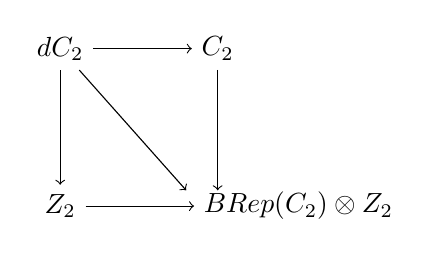
\begin{tikzpicture}
        \node (A) at (0, 2) {$\prescript{d}{}{C_2}$};
        \node (B) at (0, 0) {$\mathbb{Z}_2$};
        \node (C) at (2, 2) {$C_2$};
        \node[right] (D) at (1.7, 0) {$\text{BRep}(C_2) \otimes \mathbb{Z}_2$};
        \draw[->] (A) -- (1.6, 0.2);
        \draw[->] (A) -- (C);
        \draw[->] (A) -- (B);
        \draw[->] (B) -- (D);
        \draw[->] (C) -- (2, 0.2);
    \end{tikzpicture}
\]